\section{Evaluation}
\label{sec:eval}
\begin{center}
\begin{figure*}[ht!]
 \centering
 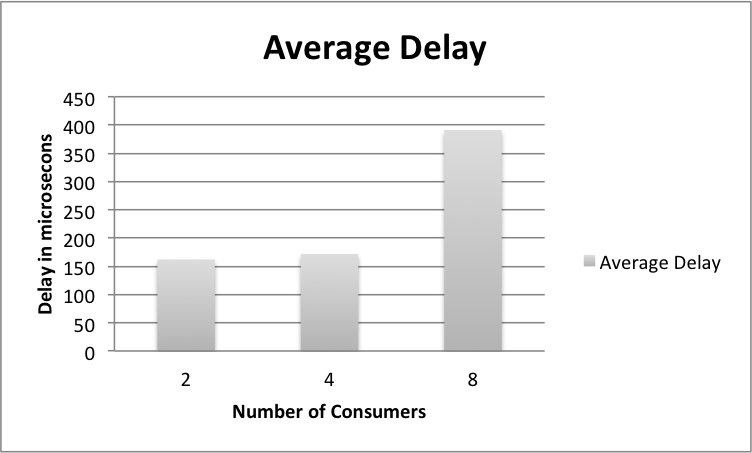
\includegraphics[width=4.0in]{avgdelay.png}
 %img1.pdf: 0x0 pixel, 300dpi, 0.00x0.00 cm, bb=
\caption{Average Delay Measurement}
\label{fig:delay}
\end{figure*}
\end{center}
\ref{nettop}.
\begin{center}
\begin{figure*}[ht!]
 \centering
 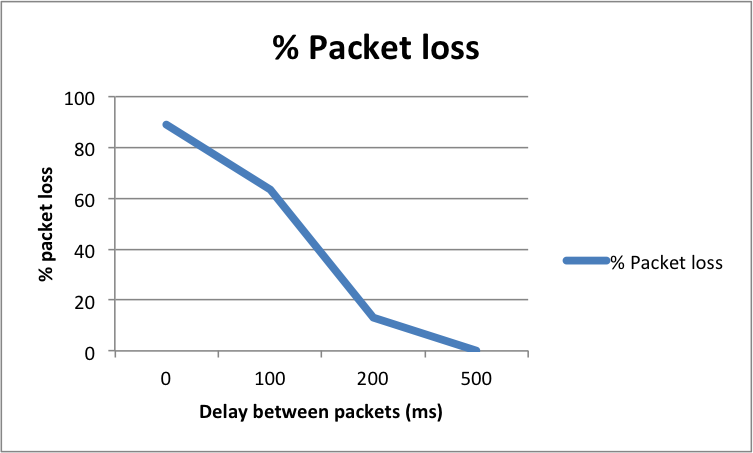
\includegraphics[width=4.0in]{packetloss.png}
 %img1.pdf: 0x0 pixel, 300dpi, 0.00x0.00 cm, bb=
\caption{Packet Loss Measurement}
\label{fig:pktloss}
\end{figure*}
\end{center}
\subsection{Experimental Setup}
Our implementation is a file sharer that uses the TRAMP platform to distribute files as described in Section \ref{sec:streamer}. We ran our experiments with one producer and 2 to 8 consumers. We ran all experiments on machines with Intel(R) Xeon(TM) CPU 3.20GHz quad core processors, 8GB RAM and connected with gigabit Ethernet. For workload we send a 55MB movie file from the producers to the consumers. The packet size is limited to 320KB to mimic the real time video streaming bit rate. However, it is possible to read multiple chunks of 320KB and fill the 32MB limit of shared memory, which is not similar to a real time application. We sent the packets from producer with 100 milliseconds delay since without this delay the consumers could not process the data and lost some packets as the tramp daemon overwrites the shared memory when the new packets arrive.






\subsection{Average Delay}
We measure the average delay by sending the packet from producer and recording a timestamp $t_1$ before sending. For the sake of measuring the delay we reply the packet back to the sender with an ACK header. After the ACK packet is received the timestamp $t_2$ is noted again and the delay is computed as the 
\[
 (t_2-t_1)/2
\]

. Since we ran experiments on machines connected with gigabit Ethernet the network delay is negligible. The total delay is measured as the sum of processing delay at producer side, the network delay and the processing delay at consumer side. We denote the delays as below:
\begin{enumerate}
 \item Processing delay at producer: $PD$
\item Processing delay at consumer: $CD$
\item Network delay: $ND$
\end{enumerate}

The total delay is given by
\[
 PD + ND + CD
\]

In Figure \label{fig:delay} we show the average delay of sending packets from the producer to the consumer. The three parts of the delay $PD$, $CD$ and $ND$, are show in three stacks. We list the observations we made in the following:
\begin{enumerate}
 \item The $PD$ and $CD$ are almost constant for any number of consumers since it is local to each node
 \item The average network delay is the most varying 
 \item The difference between 2 consumers and 4 consumers is negligible (841 and 850 micro seconds). 
  \item In case of 2 consumers the producer sends the packets to consumers in 1 hop.
 \item In case of 4 consumers 2 of the consumers received packets in 1 hop and 2 consumers received packets in 2 hops, hence the difference is negligible.
\item However in case of 8 consumers the average delay significantly increases since there was consumer which received packets in 4 hops.
\end{enumerate}

The observations we made are due to the fact that the neighbors for dissemination of packets are chosen with minimum delay neighbors as described in Section 

\subsection{Packet Loss}
As described in Section \ref{smp} if the packet send rate is significantly fast (55MB in 40252 microseconds) results in around 88\% packet loss. Even though the network is reliable the loss is due to the fact the producer is significantly fast and consumer is significantly slow to process the packets. We did some measurements for packet loss with 100 milliseconds delay before sending next packet, however the results we obtained were not meaningful due to some unknown problem. We omit the results in this paper due to lack of time. In Figure \ref{fig:delay} we show that with no delay between packets there is a packet loss of around 88\% and with 500ms delay between packets we were able to eliminate the packet loss to 0\%.

